\section{Thrust 3. Applications of {\tool}}
\label{sec:thrust3}


\subsection{Method-Level Vulnerability Detection}
%\label{mlvd:sec}

%\subsection{Problem Formulation}

Deep learning (DL)-based approaches that utilize PDGs for
vulnerability detection (VD) can tolerate a low level of errors in the
program dependencies, wherein the imprecision acts as noise and aids
in regularizing the model. VulCNN~\cite{wu2022vulcnn} is one such
state-of-the-art method-level VD tool that takes as input a program
semantics-capturing image extracted from the PDGs. In our plan,
we seek to determine how the PDGs predicted by \tool (say,
PDG\textsuperscript{*}) for {\em complete} methods affect the
performance of downstream tasks.

%We will describe another VD experiment
%for code snippets in Section~\ref{sec:fragment}.

We leverage VulCNN by taking as input both PDG\textsuperscript{*} and
the PDG derived from a program analysis tool (say,
PDG\textsuperscript{\#}) for these methods, aiming to see how closely
PDG\textsuperscript{*} mimics PDG\textsuperscript{\#} and approximates
the performance of the VD model. Mathematically, we can formulate our
task as follows:
\begin{equation}
    \centering
    0 < VD\{PDG\textsuperscript{*}\} \leq VD\{PDG\textsuperscript{\#}\}
\end{equation}
where $VD\{.\}$ indicates the performance of the automated VD model. Here, if $VD\{PDG\textsuperscript{*}\} \lesssim VD\{PDG\textsuperscript{\#}\}$, we can establish the efficacy of the PDGs from \tool for vulnerability detection.


%{\bf Data Collection}: We facilitate this study by using the VD
%dataset collected by Li {\em et al.}~\cite{yioopsla19}, which
%comprises of complete Java methods collected from eight large
%open-source Java projects.

%{\bf Experiment Setup}: For all Java methods in the~VD dataset, we
%extract program dependencies (i.e., data and control-dependence edges)
%via Joern program analysis tool~\cite{joern-2014}. Next, we leverage
%\tool that was trained on a Java dataset
%to generate the PDGs (i.e., PDG\textsuperscript{*}) for all the
%complete methods in the VD dataset. We then use
%PDG\textsuperscript{\#} and PDG\textsuperscript{*} as the input of
%VulCNN for VD.

%{\bf Evaluation Metrics}: We adopt the same metrics in Wu et
%al.~\cite{wu2022vulcnn} to evaluate VulCNN, i.e., \textit{true
%  positive rate} (TPR) (also referred to as \textit{Recall}),
%\textit{true negative rate} (TNR), and \textit{F-score}. Here, the
%positive label corresponds to the presence of a vulnerability in the
%method under study, and vice versa.

\subsection{Predictive Dynamic Slicing}

\begin{figure}[t]
\begin{center}
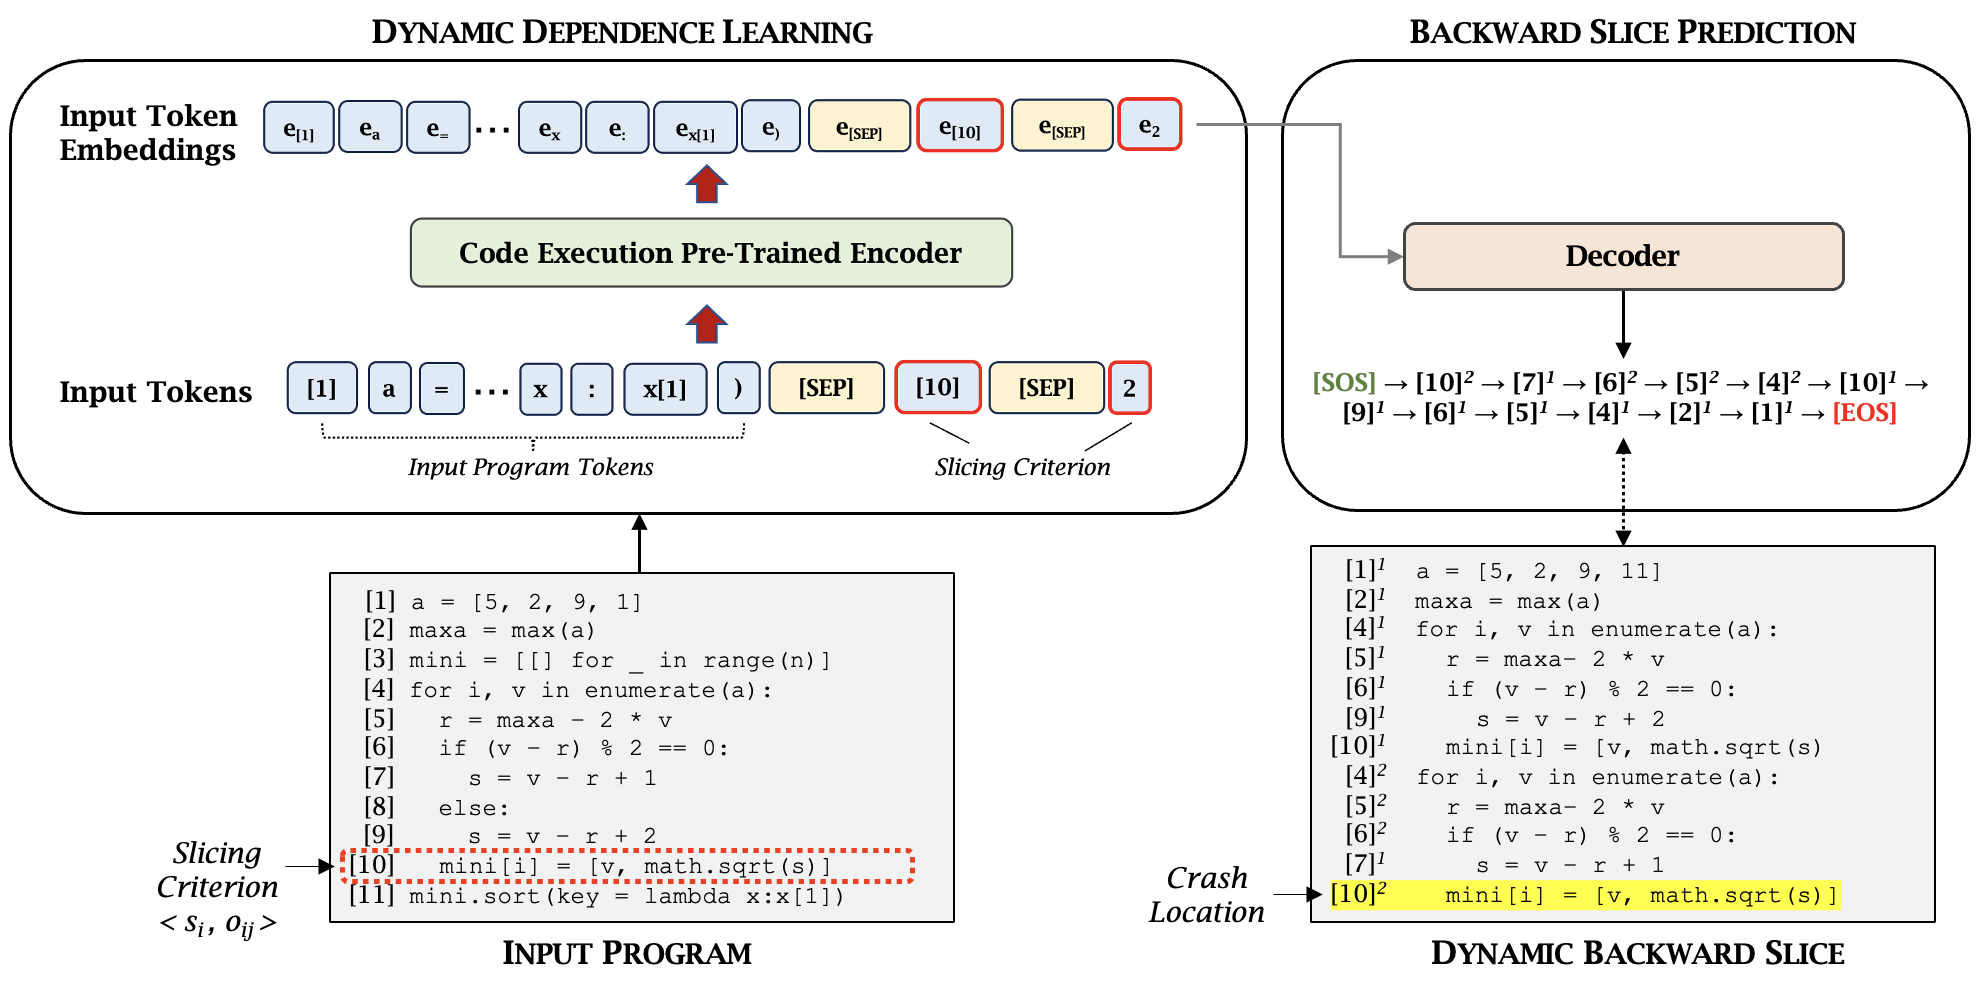
\includegraphics[width=5in]{dynamic-slicing.png}
\vspace{-12pt}
\caption{Predictive Dynamic Slicing}
\label{fig:dynamic-slicing}
\end{center}
\end{figure}

Given an (in)complete program, its inputs, and a specific statement with its occurrence in the execution trace as the slicing criterion, {\tool} predicts the dynamic backward slice for the criterion. In Fig.~\ref{fig:dynamic-slicing}, we illustrate the model architecture for {\tool}.
%Broadly, it adopts the sequence-to-sequence framework for predictive slicing, with the following essential components:
%\subsubsection{Dynamic Dependence Learning}
%In recent times, specialized source code models~\cite{icse23, graphcodebert-iclr21} have highlighted the effectiveness of learning-based approaches in understanding data and control dependencies. However, their learning objectives do not focus on run-time behavior of code, limiting their suitability for predictive slicing. To address this challenge, we chose to leverage CodeExecutor~\cite{liu2023code}, a model pre-trained on code execution, as the encoder in our framework. This code execution pre-training equips {\tool} with the capability to {\em learn dynamic program dependencies}. Furthermore, treating source code as a sequence of tokens empowers such pre-trained models (PTMs) to operate efficiently for both complete and partial code, thereby overcoming the limitations of dynamic execution, which is typically applicable only to complete code.
Let us consider a program $P = \langle s_1, s_2, \cdots, s_{N}\rangle$, where $s_i$ represents a statement in the program. Note that the inputs to the program, $I_P$, are included as assignment statements at the beginning of the program. We represent each statement $s_i$ as a sequence of code tokens \(\langle [i], t_1^{(i)}, t_2^{(i)}, \cdots, t_{M_i}^{(i)}\rangle\), where $[i]$ represents the special {\em line identifier} token included at the beginning of every line. For a given slicing criterion $\langle s_c, o \rangle$, that denotes the task of predicting the slice for the $o$-th occurrence of the statement $s_c$ in its execution history, the inputs to the encoder in {\tool} are as follows:

\begin{center}
$\{ [1], t_1^{(1)}, t_2^{(1)}, \cdots, t_{M_1}^{(1)}, \cdots, [\text{N}], t_1^{(N)}, t_2^{(N)}, \cdots, t_{M_N}^{(N)}, [\textbf{SEP}], [c], [\textbf{SEP}], o \}$
\end{center}

For each token $t$ in this input representation, the DDL module generates a contextually enriched token representation $e_t \in \mathbb{R}^d$ (where $d$ is the model dimension) with the following goals: (1) $e_t$ is syntax, semantics, and execution-aware; (2) it learns the execution-flow based on the model input tokens $t_x \in I_P$; (3) it learns the dynamic data and control dependencies between $t_j \in P$ and $t^{(c)}$ based on the occurrence of the slicing criterion denoted by $[c]$ and $o$, respectively.

\subsubsection{Backward Slice Prediction}
The primary challenge in predicting backward slices lies in ensuring that the sequence of statement/line occurrence aligns with the actual execution history, where the output sequence captures all dynamic data and control dependencies on the slicing criterion. Given the proven effectiveness of the {\em attention mechanism} in propagating information of the input sequence to the decoder within the sequence-to-sequence framework, we chose to adopt the Transformer decoder in {\tool}.

The encoder in the DDL module maps the model input to a sequence of continuous representations $\mathbf{x} = \{ e_{[1]}, e_{t_{1}^{(1)}}, \cdots, e_{[SEP]}, e_{[c]}, e_{[SEP]}, e_o \}$. Given $\mathbf{x}$, the decoder generates an output sequence $\mathbf{y} = \{y_1, y_2, \cdots, y_k\}$ of symbols one element at a time. Here, each $y_k$ corresponds to the special line identifier token $[i]$ in the input representation. This process is auto-regressive, where the previously generated symbols are consumed as the additional input for generating the next.
